\documentclass[runningheads]{llncs}
\usepackage[T1]{fontenc}
\usepackage[utf8]{inputenc}
\usepackage{lmodern} 
\usepackage{graphicx}
\usepackage{amsmath,amssymb}
\usepackage{hyperref}
\usepackage{xcolor}
\usepackage{booktabs}
\usepackage{tabularx}
\usepackage{ragged2e}
\usepackage{array}
\usepackage{ltxtable}
\usepackage{longtable}
\usepackage{cite}
\usepackage{float}

\newcolumntype{L}{>{\RaggedRight\arraybackslash}X}
\newcolumntype{P}[1]{>{\RaggedRight\arraybackslash}p{#1}}


\usepackage[section]{placeins} 
\setcounter{topnumber}{5}
\setcounter{bottomnumber}{5}
\setcounter{totalnumber}{10}
\renewcommand{\topfraction}{0.9}
\renewcommand{\textfraction}{0.07}
\renewcommand{\floatpagefraction}{0.75}
\title{Reinforcement Learning in Healthcare: A Comprehensive Review of Applications, Challenges, and Future Directions}

\author{Djelloul Daouadji Fadela \and Bachir Bouidjra Rochdi}
\institute{Department of Computer Science, University Mascara, Mascara, Algeria \\
\email{djellouldaouadji.f@univ-mascara.dz}
}

\begin{document}
\maketitle

\begin{abstract}
Reinforcement Learning (RL) is a powerful, adaptive tool for personalized healthcare decisions,
as revealed by a systematic review of many studies from 2019–2025.
The review categorized applications across intensive care, chronic disease,
diagnostics, and personalized interventions, identifying key algorithms
like DQN, PPO, and Actor-Critic methods, alongside promising hybrid models that merge clinical knowledge with RL.
While specific methods achieved high success (e.g., Supervised-Actor-Critic for sepsis with 99 accuracy), 
deployment faces critical challenges: data quality/scarcity, limited generalizability, complex reward design,
interpretability, safety/ethics, and computational constraints.
\end{abstract}

\keywords{Artificial Intelligence, Personalized Healthcare, Deep Learning, Reinforcement Learning, Predictive Analytics, Precision Medicine}

\section{Introduction}
Reinforcement learning (RL), a branch of artificial intelligence, is increasingly important in medicine due to its ability to model dynamic, sequential decision-making. Unlike traditional machine learning, RL algorithms interact with environments, adaptively learning optimal strategies through feedback. This makes RL well-suited for healthcare, where patient conditions and treatments evolve over time. RL enables personalized care by tailoring interventions to individual patient characteristics and preferences. This review provides a comprehensive overview of RL in healthcare, covering its principles, key applications, challenges, and future opportunities. We also discuss ethical and practical considerations, including data privacy, interpretability, and the need for clinical validation, aiming to highlight RL’s potential to transform patient care and outcomes~\cite{banumathiReinforcementLearningPersonalized2025,deshmukhReinforcementLearningHealthcare2024}.

Figure~\ref{fig: workflow} presents the high-level RL workflow used throughout this review; the following sections describe its components and how they map to clinical problems.
\begin{figure}[htbp]
    \centering 
    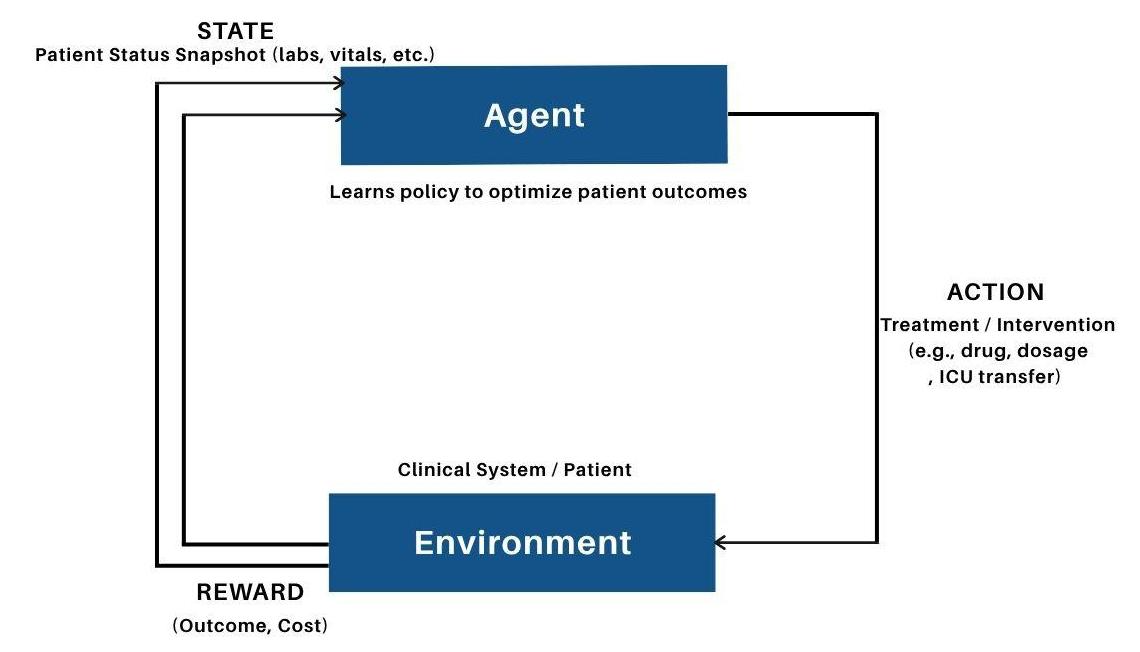
\includegraphics[width=1.0\textwidth]{figures/workflow.png} 
    \caption{Reinforcement Learning Workflow in Healthcare}
    \label{fig: workflow}
\end{figure}

\section{Related Work and Background}

Reinforcement Learning (RL) has emerged as a transformative approach in healthcare, enabling adaptive, sequential decision-making that aligns with the dynamic nature of patient care. Early RL applications focused on critical care, such as optimizing sepsis management and mechanical ventilation settings using large-scale datasets like MIMIC-III~\cite{wuValuebasedDeepReinforcement2023, yuSupervisedactorcriticReinforcementLearning2020}. These studies demonstrated that RL algorithms, including Q-learning, Deep Q-Networks (DQN), and Actor-Critic methods, can outperform traditional protocols by personalizing treatment strategies and improving patient outcomes.

Beyond critical care, RL has been applied to chronic disease management, notably in diabetes and cardiovascular diseases. For example, Q-learning and PPO have been used to personalize insulin dosing for Type 1 Diabetes~\cite{javadReinforcementLearningBased2019, zhaoSafeenhancedFullyClosedloop2025}, while Deep Q-learning has optimized warfarin dosing in cardiovascular patients~\cite{zadehOptimizingWarfarinDosing2023}. These approaches leverage patient-specific data to tailor interventions, demonstrating improved accuracy and clinical concordance.

In medical diagnostics, RL has shown promise in enhancing image-based disease detection and localization. Studies using DQN and CNNs have improved skin cancer classification on the HAM10000 dataset~\cite{barataReinforcementLearningModel2023}, and enabled accurate brain tumor localization in MRI scans with minimal training data~\cite{stemberReinforcementLearningUsing2022}. RL-based models have also been developed for disease prediction using electronic health records (EHRs), achieving higher accuracy than conventional machine learning methods~\cite{abdelazizDeepQNetworkDQN2025}.

Recent work has expanded RL’s scope to personalized interventions, such as medication adherence and digital health recommendations. Contextual bandit RL and wearable-based adaptive interventions have been used to deliver real-time, patient-specific guidance, improving engagement and outcomes~\cite{ismailAdvancingPatientCare2024, tripathyReinforcementLearningOptimizing2024}.

Despite these advances, several challenges persist. RL models often require large, high-quality datasets, yet many healthcare studies rely on limited or simulated data, which can affect generalizability. Interpretability remains a concern, as complex RL models may act as “black boxes,” hindering clinical trust and adoption. Designing clinically meaningful reward functions, ensuring patient safety during exploration, and integrating RL systems into real-world clinical workflows are ongoing areas of research.


Overall, the literature highlights RL’s potential to revolutionize healthcare by enabling personalized, data-driven decision-making. However, further work is needed to address data limitations, improve model transparency, and validate RL approaches in prospective clinical trials.

\subsection*{Summary and gaps}
While RL has demonstrated promising results across diverse healthcare domains, persistent gaps remain in interpretability, clinical validation, and integration with real-world workflows. This review addresses these gaps by systematically categorizing RL applications, identifying key challenges, and proposing future research directions to advance safe and effective RL deployment in healthcare.


\section{RL Applications in Healthcare: A Taxonomy}
This section organizes RL applications into a compact taxonomy and then surveys representative works for each category.

Figure~\ref{fig: timeline} provides a concise timeline of notable RL applications (2019--2025) discussed below.

\begin{figure}[htbp]
    \centering 
    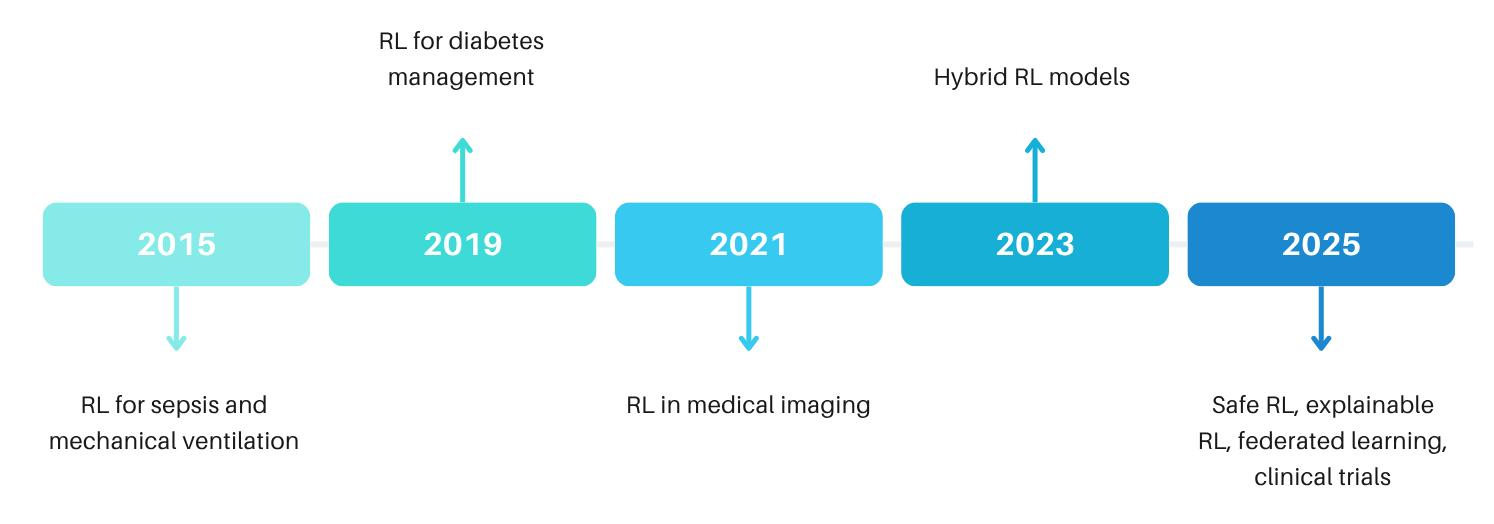
\includegraphics[width=1.0\textwidth]{figures/timeline.png} 
    \caption{Timeline of RL Applications in Healthcare (2019-2025)}
    \label{fig: timeline}
\end{figure}
\subsection{Intensive Care and Critical Care}

\subsubsection{Sepsis Treatment}
Multiple studies address sepsis management through optimal dosing of IV fluids and vasopressors. Notable approaches include:
\begin{itemize}
    \item \textbf{WD3QNE}: Weighted Dueling Double DQN with embedded human expertise using conditional policies based on SOFA scores~\cite{wuValuebasedDeepReinforcement2023}
    \item \textbf{DDPG-based approaches}: Continuous action spaces for fine-grained dosing control~\cite{linDosingStrategyModel2022}
    \item \textbf{Representation learning}: Neural CDEs for encoding sequential observations~\cite{killianEmpiricalStudyRepresentation2020}
    \item \textbf{Policy evaluation and reward design}: Challenges and best practices discussed in~\cite{luoReinforcementLearningDynamic2024,zhangReinforcementLearningClinical2019}
\end{itemize}

\subsubsection{Mechanical Ventilation and Sedation}
Supervised-Actor-Critic (SAC) combines long-term RL objectives with short-term supervised learning to align with clinical practices, achieving 99\% accuracy and faster convergence than traditional Actor-Critic methods on MIMIC-III data (8,860 patients)~\cite{yuSupervisedactorcriticReinforcementLearning2020}. RL has also been used for ventilator setting optimization~\cite{liuReinforcementLearningOptimize2024}.

\subsection{Chronic Disease Management}

\subsubsection{Diabetes Management}
\begin{itemize}
    \item \textbf{Type 1 Diabetes}: Q-learning for insulin dosing~\cite{javadReinforcementLearningBased2019}, PPO for artificial pancreas achieving 87\% time-in-range~\cite{zhaoSafeenhancedFullyClosedloop2025}
    \item \textbf{Type 2 Diabetes}: Clustered DQN for precision medicine with 81-85\% clinician concordance~\cite{ohEffectiveDatadrivenPrecision2022}
\end{itemize}

\subsubsection{Cardiovascular Diseases}
Warfarin dosing optimization using Deep Q-learning on PK/PD simulations, outperforming clinical protocols in maintaining therapeutic INR ranges~\cite{zadehOptimizingWarfarinDosing2023}.

\subsection{Diagnostic and Prediction Systems}

\subsubsection{Medical Imaging}
\begin{itemize}
    \item \textbf{Skin Cancer}: CNN+DQN achieving 80\% accuracy on HAM10000 dataset~\cite{dahdouhNewApproachUsing2023,barataReinforcementLearningModel2023}
    \item \textbf{Brain Tumors}: DQN for tumor localization achieving 70\% accuracy vs. 11\% supervised baseline~\cite{stemberReinforcementLearningUsing2022}
\end{itemize}

\subsubsection{Disease Prediction}
Deep Attention Q-Networks with Transformers for critical care recommendations, outperforming LSTM and traditional RL baselines~\cite{maDeepAttentionQnetwork2023}. DQN models have also been used for disease prediction from EHRs~\cite{abdelazizDeepQNetworkDQN2025}.

\subsection{Personalized Interventions}

\subsubsection{Medication Adherence}
Contextual Bandit RL combined with CNN verification for personalized engagement and error minimization in medication taking~\cite{ismailAdvancingPatientCare2024}.

\subsubsection{Digital Health Interventions}
Wearable-based adaptive interventions using Deep Q-Learning for real-time, context-aware recommendations~\cite{tripathyReinforcementLearningOptimizing2024,gonulReinforcementLearningBased2021,hassouniClusteringbasedReinforcementLearning2020}.

We summarize the domain-level taxonomy in Figure~\ref{fig: taxonomy} and then detail the main subareas (intensive care, chronic disease, diagnostics, personalized interventions).
\begin{figure}[htbp]
    \centering 
    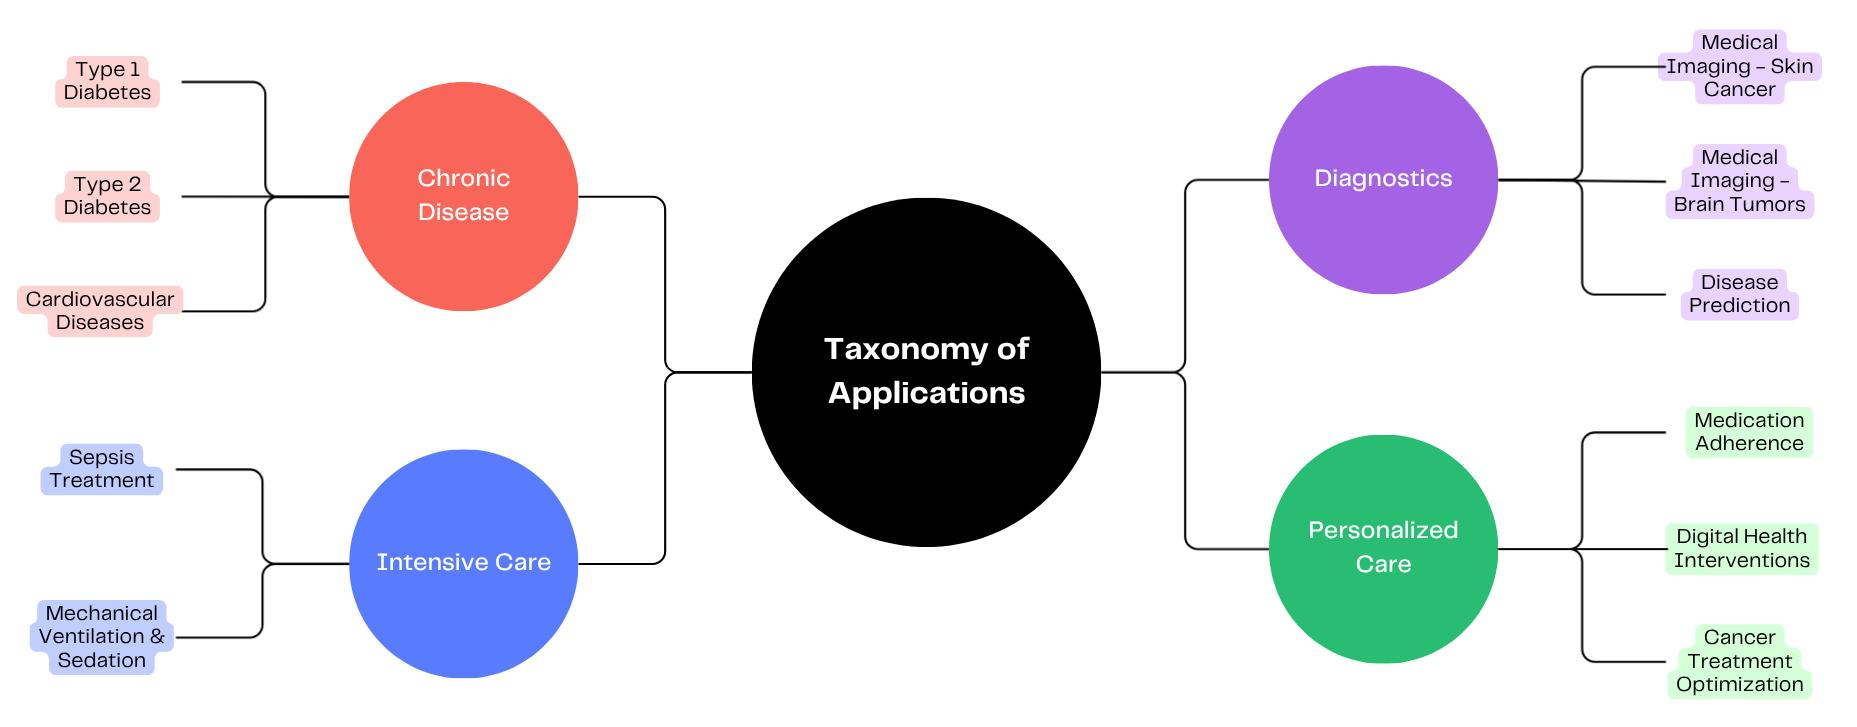
\includegraphics[width=1.0\textwidth]{figures/taxonomy.png} 
    \caption{Taxonomy of RL Applications in Healthcare}
    \label{fig: taxonomy}
\end{figure}
\section{Datasets Used in RL Healthcare Studies} 
Below table lists commonly used datasets and their typical applications in RL healthcare research.

\begin{table}[htbp]
\centering
\caption{RL Healthcare Articles Grouped by Dataset Type}
\label{tab:datasets}
\begin{tabular}{|p{3cm}|p{5cm}|p{5cm}|}
\hline
\textbf{Dataset} & \textbf{Clinical Domain / Application} & \textbf{References} \\
\hline
MIMIC-III & Sepsis, mechanical ventilation, critical care, representation learning & \cite{killianEmpiricalStudyRepresentation2020, linDosingStrategyModel2022,luoReinforcementLearningDynamic2024,wuValuebasedDeepReinforcement2023, yuSupervisedactorcriticReinforcementLearning2020, liuReinforcementLearningOptimize2024, maDeepAttentionQnetwork2023} \\
\hline
HAM10000 & Dermatology, skin cancer classification & \cite{barataReinforcementLearningModel2023,dahdouhNewApproachUsing2023} \\
\hline
UCI Heart Disease & Heart disease prediction, EHR-based disease prediction & \cite{gayathriEnhancingHeartDisease2024,abdelazizDeepQNetworkDQN2025} \\
\hline
HeartSteps & Physical activity e-Health interventions & \cite{hassouniClusteringbasedReinforcementLearning2020} \\
\hline
MGH T1DM Patient Records & Insulin dosing for T1DM & \cite{javadReinforcementLearningBased2019} \\
\hline
Custom/Simulated Data & Sepsis simulation, digital interventions, closed-loop healthcare, e-Health & \cite{petersenDeepReinforcementLearning2019,gonulReinforcementLearningBased2021, daiClosedloopHealthcareProcessing2022, hassouniClusteringbasedReinforcementLearning2020} \\
\hline
WEA App (Asthma) & Asthma exacerbation prediction & \cite{aliyuReinforcementLearningApproach2025} \\
\hline
BraTS MRI & Brain tumor localization & \cite{stemberReinforcementLearningUsing2022} \\
\hline
NYU Langone EHR & T2DM multimorbidity management & \cite{zhengPersonalizedMultimorbidityManagement2021} \\
\hline
NHISS EHR (Korea) & T2DM precision medicine & \cite{ohEffectiveDatadrivenPrecision2022} \\
\hline
MD Anderson Cancer Center & Oropharyngeal cancer treatment & \cite{tardiniOptimalTreatmentSelection2022} \\
\hline
TCGA, GDSC, Immunohistochemistry & Cancer drug ranking & \cite{liuDeepReinforcementLearning2022} \\
\hline
Samsung Smartwatch / Wearables & Wearable-based interventions & \cite{tripathyReinforcementLearningOptimizing2024} \\
\hline
Simglucose Simulator (FDA UVa/Padova) & Artificial pancreas (T1D) & \cite{zhaoSafeenhancedFullyClosedloop2025} \\
\hline
PK/PD Simulation & Warfarin dosing, Erdafitinib dosing & \cite{zadehOptimizingWarfarinDosing2023,decarloReinforcementLearningPKPD2024} \\
\hline
\end{tabular}
\end{table}

\FloatBarrier
\begin{figure}[htbp]
  \centering
    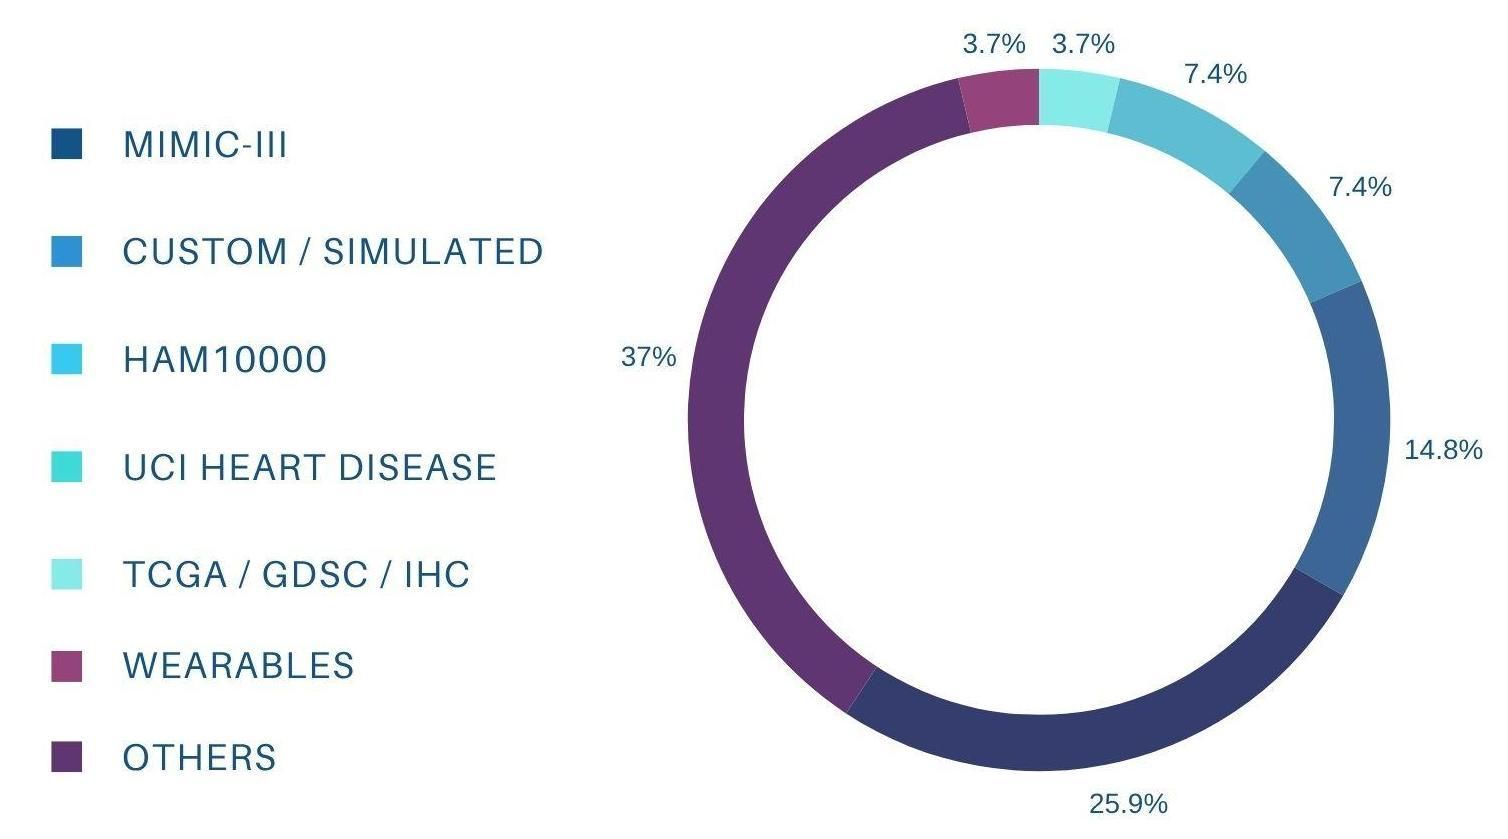
\includegraphics[width=0.8\textwidth]{figures/dataset.jpg} 
    \caption{Distribution of Datasets Used in RL Healthcare Studies}
    \label{fig: dataset_pie_chart}
\end{figure}
\section{Challenges in Reinforcement Learning for Personalized Medicine}
This section summarizes key barriers to deploying RL in clinical settings and highlights areas where methodological work is most needed.

\begin{itemize}
    \item \textbf{Data Quality and Availability:} Clinical datasets are often limited, noisy, incomplete, or imbalanced, which hinders robust RL model training and generalization \cite{yangDeepReinforcementLearning2024, killianEmpiricalStudyRepresentation2020, deshmukhReinforcementLearningHealthcare2024, luoReinforcementLearningDynamic2024, barataReinforcementLearningModel2023, hassouniClusteringbasedReinforcementLearning2020, mulaniDeepReinforcementLearning2020}.
    \item \textbf{Generalizability and Bias:} Models trained on single-center or homogeneous datasets may not generalize to diverse populations, raising concerns about fairness and bias \cite{ohEffectiveDatadrivenPrecision2022, banumathiReinforcementLearningPersonalized2025, banumathiReinforcementLearningPersonalized2025a, zadehOptimizingWarfarinDosing2023, zhengPersonalizedMultimorbidityManagement2021}.
    \item \textbf{Interpretability and Transparency:} Deep RL models are often ``black boxes,'' making it difficult for clinicians to understand, trust, and validate recommendations \cite{maDeepAttentionQnetwork2023, deshmukhReinforcementLearningHealthcare2024, barataReinforcementLearningModel2023, wuValuebasedDeepReinforcement2023, frommeyerReinforcementLearningIts2025, banumathiReinforcementLearningPersonalized2025}.
    \item \textbf{Reward Function Design:} Defining clinically meaningful, multi-objective reward functions that align with patient outcomes, safety, and quality of life is complex \cite{luoReinforcementLearningDynamic2024, frommeyerReinforcementLearningIts2025, petersenDeepReinforcementLearning2019, yangPrescDRLDeepReinforcement2024, zadehOptimizingWarfarinDosing2023}.
    \item \textbf{Safety and Ethics:} RL exploration can pose risks to patient safety; ethical constraints and regulatory requirements limit the scope of experimentation \cite{zhaoSafeenhancedFullyClosedloop2025, deshmukhReinforcementLearningHealthcare2024, mulaniDeepReinforcementLearning2020, gorrepatiReinforcementLearningFramework2025, yuSupervisedactorcriticReinforcementLearning2020}.
    \item \textbf{Computational Complexity and Scalability:} Training RL models on high-dimensional, multimodal clinical data requires significant computational resources and expertise \cite{DOI105425427552721, hassouniClusteringbasedReinforcementLearning2020, gorrepatiReinforcementLearningFramework2025, yangDeepReinforcementLearning2024}.
    \item \textbf{Offline Policy Evaluation and Validation:} Reliable evaluation of RL policies using retrospective data is challenging due to confounding, delayed effects, and lack of ground truth \cite{luoReinforcementLearningDynamic2024, killianEmpiricalStudyRepresentation2020, zhengPersonalizedMultimorbidityManagement2021, zadehOptimizingWarfarinDosing2023}.
    \item \textbf{Integration with Clinical Workflows:} Embedding RL systems into real-world clinical practice requires overcoming technical, regulatory, and workflow barriers \cite{barataReinforcementLearningModel2023, ohEffectiveDatadrivenPrecision2022, gorrepatiReinforcementLearningFramework2025, banumathiReinforcementLearningPersonalized2025}.
\end{itemize}
Figure~\ref{fig: challenges} illustrates the principal challenge categories that we discuss below.
\begin{figure}[h]
    \centering 
    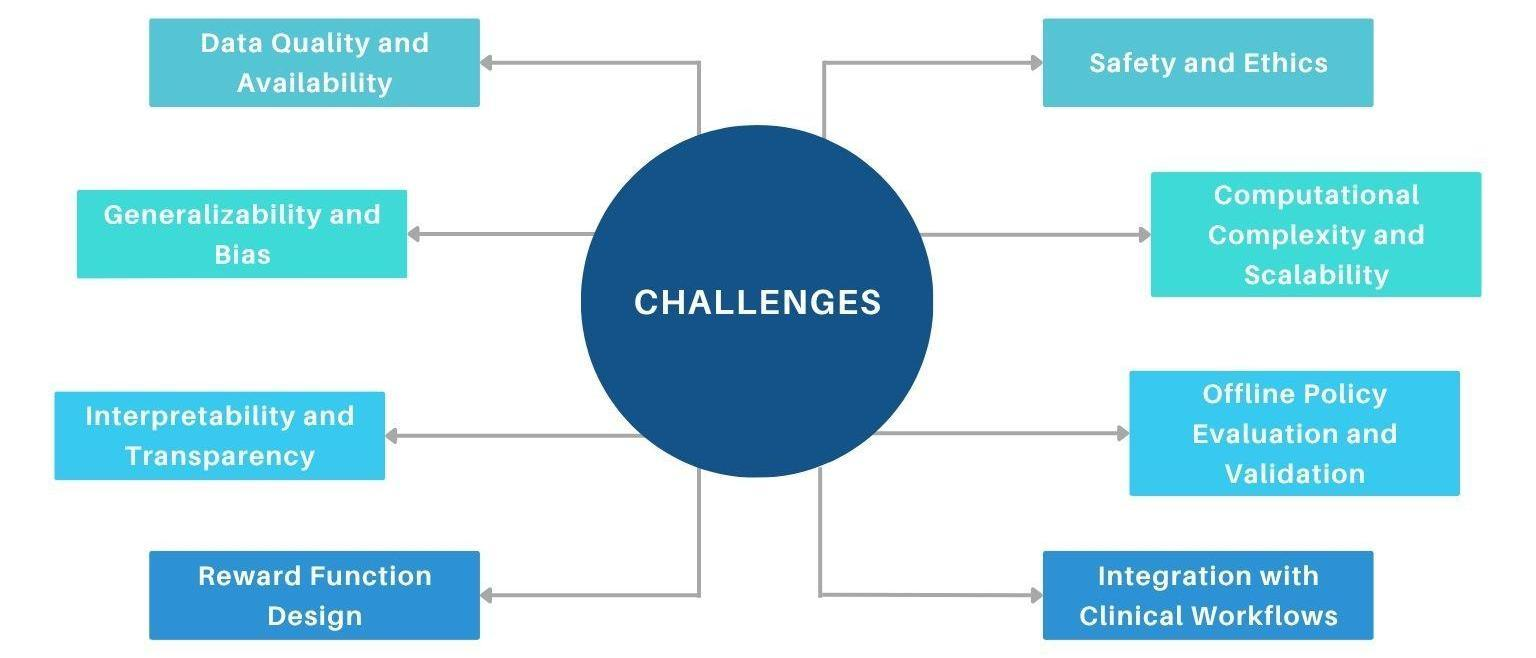
\includegraphics[width=1.0\textwidth]{figures/challenges.jpg} 
    \caption{Key Challenges in Reinforcement Learning for Personalized Medicine}
    \label{fig: challenges}
\end{figure}

\section{Future Works and Directions}
To address these challenges, future research should focus on:

\begin{itemize}
    \item \textbf{Model Interpretability and Explainability:} Develop explainable RL models using XAI techniques (e.g., SHAP, LIME, attention mechanisms) to build clinician trust and facilitate adoption \cite{banumathiReinforcementLearningPersonalized2025, maDeepAttentionQnetwork2023, gorrepatiReinforcementLearningFramework2025, frommeyerReinforcementLearningIts2025}.
    \item \textbf{Federated and Privacy-Preserving Learning:} Employ federated RL and privacy-preserving data sharing to enable multi-center collaboration while protecting patient privacy \cite{banumathiReinforcementLearningPersonalized2025, abdellatifReinforcementLearningIntelligent2021, banumathiReinforcementLearningPersonalized2025a}.
    \item \textbf{Hybrid and Safe RL Algorithms:} Integrate supervised learning, expert knowledge, and safety constraints into RL frameworks to ensure reliable and clinically aligned decision-making \cite{wuValuebasedDeepReinforcement2023, yuSupervisedactorcriticReinforcementLearning2020, zhaoSafeenhancedFullyClosedloop2025, gorrepatiReinforcementLearningFramework2025}.
    \item \textbf{Advanced RL Methods:} Explore meta-RL, hierarchical RL, multi-agent RL, and digital twin simulations for more robust, adaptive, and personalized treatment strategies \cite{banumathiReinforcementLearningPersonalized2025, decarloReinforcementLearningPKPD2024, gorrepatiReinforcementLearningFramework2025, petersenDeepReinforcementLearning2019}.
    \item \textbf{Clinical Validation and Real-World Trials:} Move beyond retrospective studies to prospective, real-time clinical trials and integration with electronic medical record (EMR) systems \cite{zhengPersonalizedMultimorbidityManagement2021, gorrepatiReinforcementLearningFramework2025, barataReinforcementLearningModel2023, ohEffectiveDatadrivenPrecision2022}.
    \item \textbf{Reward Function Refinement:} Design multi-objective, patient-centered reward functions that balance efficacy, safety, cost, and quality of life \cite{luoReinforcementLearningDynamic2024, petersenDeepReinforcementLearning2019, yangPrescDRLDeepReinforcement2024, zadehOptimizingWarfarinDosing2023}.
    \item \textbf{Interdisciplinary Collaboration:} Foster collaboration among AI researchers, clinicians, ethicists, and policymakers to ensure responsible, effective, and ethical RL system design \cite{banumathiReinforcementLearningPersonalized2025, banumathiReinforcementLearningPersonalized2025a, frommeyerReinforcementLearningIts2025}.
    \item \textbf{Standardized Benchmarks and Taxonomies:} Develop standardized datasets, benchmarks, and taxonomies to improve reproducibility, comparability, and clinical relevance of RL research in healthcare \cite{frommeyerReinforcementLearningIts2025, abdellatifReinforcementLearningIntelligent2021}.
\end{itemize}

\section{Conclusion}
Reinforcement learning has shown significant promise in healthcare, enabling adaptive, personalized interventions across critical care, chronic disease management, diagnostics, and digital health. Key RL algorithms, such as DQN, PPO, and Actor-Critic, have achieved high accuracy and clinical concordance in various applications. However, challenges persist in data quality, generalizability, interpretability, reward design, safety, and integration with clinical practice. Addressing these issues through explainable models, federated learning, hybrid approaches, and rigorous clinical validation will be essential for RL’s successful adoption in medicine. Continued interdisciplinary collaboration and standardized benchmarks will further support the development of robust, ethical, and impactful RL systems, ultimately improving patient outcomes and advancing precision medicine.

\bibliographystyle{splncs04}
\bibliography{references}

\end{document}